\section{Introduction}
\label{sec:introduction}

Structural heart disease includes abnormalities of ventricular function, myocardial structure, and valvular function, and its confirmation and classification commonly depend on imaging examinations such as echocardiography\cite{lang2015chamber,otto2021valvular}. The 12-lead ECG is inexpensive and widely available in clinical workflows, whereas echocardiography is resource-intensive and not always accessible at the point of care. SHD frequently remains undiagnosed before cardiac imaging\cite{poterucha2025echonext}. Research on artificial intelligence-enhanced ECG (AI-ECG) shows that waveforms encode predictive information about latent structural abnormalities that is difficult to identify consistently by visual interpretation\cite{siontis2021aiecg}. Detecting echocardiography-defined SHD from ECGs therefore offers a basis for prioritizing patients who may benefit from further assessment, particularly when echocardiographic capacity is limited.

Previous deep-learning studies have used ECG waveforms or images to identify left ventricular systolic dysfunction, valvular disease, and broader echocardiographic abnormalities\cite{attia2019contractile,elias2022valvenet,ulloacerna2022rechommend,poterucha2025echonext,dhingra_present_shd_2025,aminorroaya_adapt_shd_2025}. These studies connect electrical measurements with structural phenotypes across different cohorts, input representations, and prediction targets\cite{avula2023ecgreview}. Their reliance on paired ECG--echocardiography labels motivates learning reusable representations from unlabeled waveforms.

Supervised AI-ECG models generally require consistently defined ECG--echocardiography pairs. EchoNext provides ECG records paired with binary abnormality labels derived from echocardiography\cite{elias2026echonextdata}. Compared with routinely accumulated unlabeled waveforms, the paired records available for training specific echocardiography-defined abnormality targets are constrained by this label-construction process. Masked ECG pretraining studies have therefore begun to evaluate limited-label settings as a distinct problem\cite{sawano_masked_lvsd_2024,ran_joint_masking_2024}. The central questions are whether unlabeled waveforms provide a transferable initialization and whether that initialization reduces the amount of paired labeled data required under a matched downstream protocol.

ECG self-supervised learning has explored cross-view contrastive objectives and lead-relation modeling\cite{kiyasseh2021clocs,mehari2022ssl,oh2022leadagnostic}, as well as time--lead transformation recognition and masked reconstruction\cite{zhang_reverse_2023,zhang2023maefe,na2024stmem,ran_joint_masking_2024}. Masked pretraining has been evaluated for left ventricular systolic dysfunction and in limited-label settings\cite{sawano_masked_lvsd_2024}, while foundation-model benchmarks indicate that downstream gains depend on architecture and task\cite{almasud2026benchmark}. We formulate SHD detection from synchronized 12-lead ECGs as a 12-target multi-label binary classification task. We test whether convolutional masked pretraining improves discrimination over random initialization under matched downstream architecture and training. We also assess how this difference changes with label availability.

We developed ECG-FCMAE by adapting fully convolutional masked autoencoding to synchronized 12-lead ECGs. A shared temporal-patch mask hides the same intervals in all leads, so each observed segment retains the synchronized multilead representation. It also prevents an interval masked in one lead from remaining directly visible in another lead. The transferred encoder combines a one-dimensional ConvNeXt backbone with efficient channel attention, multiscale temporal pooling, and conditioning on seven tabular variables\cite{liu2022convnext,woo2023convnextv2,wang2020ecanet,perez2018film}. Figure~\ref{fig:architecture} presents the pretraining and downstream architecture.

We compare pretrained and randomly initialized models with identical architecture, inputs, data splits, optimization, and model selection to isolate the effect of initialization. We then evaluate label efficiency across five fractions of labeled training records. Finally, we examine whether tabular conditioning contributes to downstream performance, how performance varies across the 12 prediction targets, and how reducing the available leads affects SHD discrimination.

\section{Materials and methods}
\label{sec:methods}

\subsection{Dataset and cohort}
\label{sec:cohort}

The analysis uses the released predefined splits from the EchoNext paired ECG--echocardiography cohort\cite{elias2026echonextdata}. The dataset documentation assigns specific abnormality labels to ECG records obtained within one year before echocardiography and derives negative SHD labels from records whose subsequent echocardiogram did not meet the SHD definition.

The training, validation, and test sets contained $72{,}475$, $4{,}626$, and $5{,}442$ ECG records from $26{,}218$, $4{,}626$, and $5{,}442$ patients, respectively (Table~\ref{tab:cohort}). Patient sets did not overlap across splits. A patient could contribute multiple records to the training set, whereas the validation and test sets contained one record per patient. A further $17{,}457$ records outside the predefined splits were not used. Model development and selection used the training and validation sets only, and the test set was evaluated after model selection. Figure~\ref{fig:study_design} summarizes the cohort, transfer pathway, and evaluation framework.

\begin{table}[!htbp]
\centering
\BSPCtableformat

\caption{Predefined cohort splits. Patients could contribute repeated records to the training set, whereas the validation and test sets contained one record per patient.}
\label{tab:cohort}
\begin{tabular}{lrr}
\toprule
Split & ECG records & Patients \\
\midrule
Training & 72,475 & 26,218 \\
Validation & 4,626 & 4,626 \\
Test & 5,442 & 5,442 \\
\bottomrule
\end{tabular}

\end{table}

\begin{bspcwidefigure}[!t]
\centering
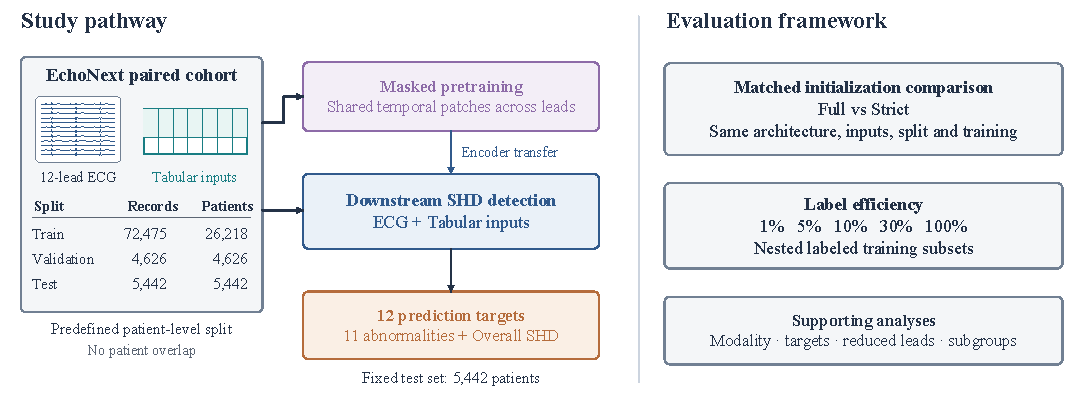
\includegraphics[width=\textwidth]{fig1_study_pathway_en.pdf}
\caption{Study pathway and evaluation framework. The retrospective EchoNext paired ECG--echocardiography cohort was partitioned at the patient level into training, validation, and test sets. Twelve-lead ECGs from the training set underwent masked self-supervised pretraining with a shared temporal mask across leads, and the resulting initialization was transferred to the downstream SHD model incorporating seven tabular variables; echocardiography was used only to define the ground-truth labels. The model produced 12 target-specific outputs comprising 11 specific abnormalities and Overall SHD. Evaluation included a matched comparison of pretrained and random initialization, label-efficiency analyses using 1\%, 5\%, 10\%, 30\%, and 100\% of the labeled training data, and supporting analyses of modality/tabular information, individual prediction targets, and reduced-lead settings.}
\label{fig:study_design}
\end{bspcwidefigure}

\subsection{Prediction targets and ground-truth label definitions}
\label{sec:outcomes}

The model simultaneously predicted 11 specific echocardiography-defined abnormalities and Overall SHD\cite{elias2026echonextdata}. The 11 abnormality criteria were LVEF $\leq45\%$; maximum diastolic thickness of the interventricular septum or left ventricular posterior wall $\geq13$~mm; moderate-or-greater aortic stenosis; moderate-or-greater aortic regurgitation; moderate-or-greater mitral regurgitation; moderate-or-greater tricuspid regurgitation; moderate-or-greater pulmonary regurgitation; moderate-or-greater right ventricular systolic dysfunction; moderate or large pericardial effusion; PASP $\geq45$~mmHg; and TR Vmax $\geq3.2$~m/s. Let $y_k\in\{0,1\}$ denote the ground-truth label for the $k$th specific abnormality, and let $y_{\mathrm{SHD}}\in\{0,1\}$ denote the ground-truth Overall SHD label. The Overall SHD label was defined as
\begin{equation}
y_{\mathrm{SHD}}=\max\{y_1,y_2,\ldots,y_{11}\}.
\label{eq:overall_shd}
\end{equation}
The Overall SHD label was positive when at least one specific abnormality label was positive and negative when all 11 labels were negative. The final classification layer outputs a 12-dimensional logit vector, with one element per prediction target. An element-wise sigmoid yields the corresponding probabilities, including a dedicated Overall SHD probability from its own logit.

\subsection{ECG and tabular inputs}
\label{sec:inputs}

Each ECG was represented by a released NPY waveform, with input tensor $\mathbf{X}\in\mathbb{R}^{12\times2500}$. The dataset documentation describes lead-wise median filtering, clipping at the 0.1st and 99.9th percentiles, and normalization using dataset-wide means and standard deviations before release. The loader converts these arrays to channel-first 32-bit floating-point tensors and preserves their released filtering, sampling, and normalization.

The tabular input comprised sex, age, ventricular rate, atrial rate, PR interval, QRS duration, and corrected QT interval (QTc). According to the dataset documentation, continuous variables were standardized before release; missing values were generally median-imputed, with missing atrial-rate and PR-interval values set to zero. Female and male were encoded as 0 and 1. The model reads the released seven-dimensional arrays and combines them with ECG representations.

\subsection{FCMAE-inspired masked ECG pretraining}
\label{sec:pretraining}

Pretraining used a masked-autoencoding reconstruction objective inspired by fully convolutional masked autoencoders (FCMAE), retaining convolutional encoding and decoding\cite{he2022mae,woo2023convnextv2}. The input was divided along time into patches of 25 samples, and 60\% of temporal patches were masked at random. The same temporal mask was applied to all 12 leads, and masked positions were set to zero at the encoder input. Sharing the temporal mask withheld each selected interval across all leads, while retaining synchronized multilead observations in the unmasked intervals.

The encoder output ($512\times78$) was projected by a $1\times1$ convolution to $256\times78$. A learned mask token replaced features at masked temporal positions. Two 256-channel ConvNeXt blocks and layer normalization preserved this shape; linear interpolation then restored 2,500 temporal positions, and a $1\times1$ convolution produced the $12\times2500$ reconstruction. Target patches were standardized within the pretraining objective, and mean squared error was calculated only over the masked set $\mathcal{M}$:
\begin{equation}
\mathcal{L}_{\mathrm{rec}}=
\frac{1}{|\mathcal{M}|}
\sum_{(c,t)\in\mathcal{M}}
\left(\hat{x}_{c,t}-\tilde{x}_{c,t}\right)^2,
\label{eq:pretrain_loss}
\end{equation}
where $\hat{x}_{c,t}$ is the reconstruction and $\tilde{x}_{c,t}$ is the standardized target. Pretraining ran for 100 epochs with AdamW, a learning rate of $1.5\times10^{-4}$, weight decay of 0.05, and a batch size of 64. Downstream models were initialized with the epoch-97 encoder parameters; the decoder served the pretraining reconstruction task.

\begin{bspcwidefigure}[!t]
\centering
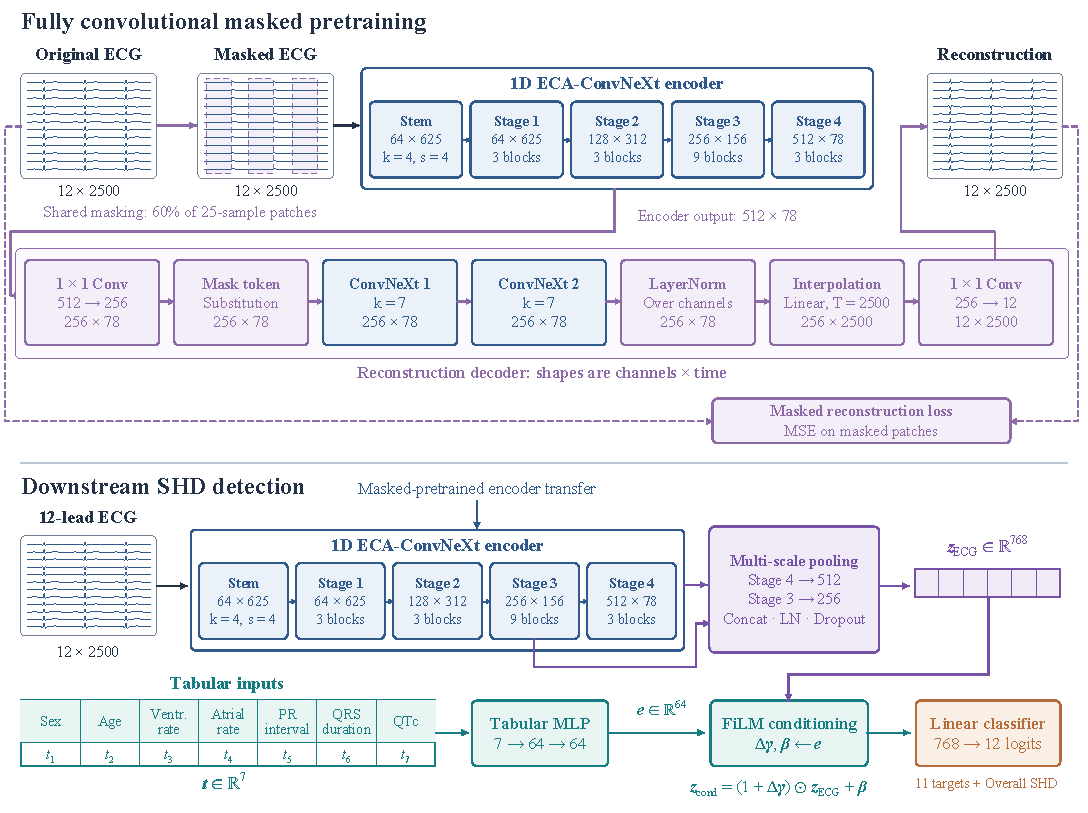
\includegraphics[width=\textwidth]{fig2_architecture_revised.pdf}
\caption{Masked pretraining and downstream architecture. During pretraining, synchronized 12-lead ECGs ($12\times2500$ samples) were divided into 25-sample temporal patches; 60\% of patch positions were masked with the same temporal mask across all leads. A one-dimensional ECA--ConvNeXt encoder and lightweight 256-channel decoder reconstructed standardized targets at masked positions using mean squared error. Pretraining ran for 100 epochs, and the epoch-97 encoder checkpoint was transferred. During downstream training, the encoder produced feature maps of $64\times625$, $128\times312$, $256\times156$, and $512\times78$. Separate temporal-attention pooling of Stages 3 and 4 yielded 256- and 512-dimensional vectors that were concatenated into a 768-dimensional ECG representation. A two-layer multilayer perceptron mapped seven tabular variables to 64 dimensions, and a linear layer generated 768-dimensional scale-offset and shift vectors. FiLM applied $(\mathbf{1}+\Delta\boldsymbol{\gamma})\odot\mathbf{z}_{\mathrm{ECG}}+\boldsymbol{\beta}$ before the final classification layer, which output a 12-dimensional logit vector. A dedicated logit yielded the Overall SHD probability. ECG traces depict three schematic cycles; the model input remains $12\times2500$. Shapes omit the batch dimension, and tabular cells denote input features.}
\label{fig:architecture}
\end{bspcwidefigure}

\subsection{One-dimensional ECA--ConvNeXt encoder}
\label{sec:encoder}

The downstream ECG encoder adapts the convolutional structure of ConvNeXt V2 to one dimension\cite{liu2022convnext,woo2023convnextv2}. A one-dimensional stem convolution with kernel size and stride 4 maps the 12 input leads to 64 channels. The four stages contain $(3,3,9,3)$ blocks with $(64,128,256,512)$ channels, producing temporal lengths of 625, 312, 156, and 78. DropPath probabilities increase linearly from 0 to 0.1 across the 18 blocks, and LayerScale is not used.

Each block applies a depthwise convolution with kernel size 7, layer normalization, a pointwise expansion by a factor of four, GELU, global response normalization (GRN), and a pointwise projection. Efficient channel attention (ECA) averages over time, models local cross-channel relationships with a one-dimensional convolution of kernel size 5, and rescales the features with sigmoid weights\cite{wang2020ecanet}. A block is written as
\begin{equation}
\mathbf{Z}_{l+1}=\mathbf{Z}_{l}+
\mathrm{DropPath}\!\left(\mathrm{ECA}\!\left[f_l(\mathbf{Z}_{l})\right]\right),
\label{eq:convnext_block}
\end{equation}
where $f_l(\cdot)$ denotes the $l$th one-dimensional ConvNeXt-V2 transformation.

Figure~\ref{fig:module_details} details the ECA--ConvNeXt block, channel attention, multiscale temporal pooling, and tabular conditioning.

\begin{bspcwidefigure}[!t]
\centering
\begin{minipage}[t]{0.49\textwidth}
  \centering
  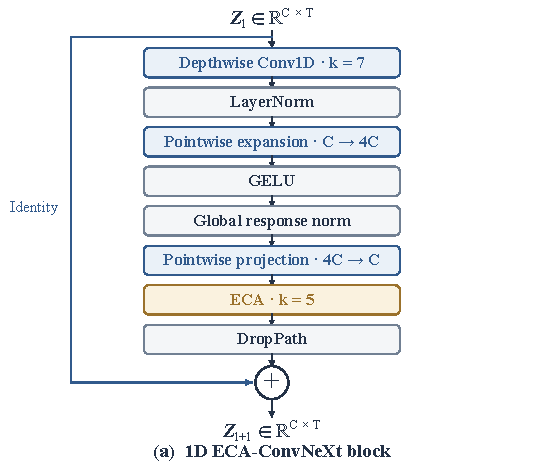
\includegraphics[width=\linewidth]{fig3a_eca_convnext_block_revised.pdf}
\end{minipage}\hfill
\begin{minipage}[t]{0.49\textwidth}
  \centering
  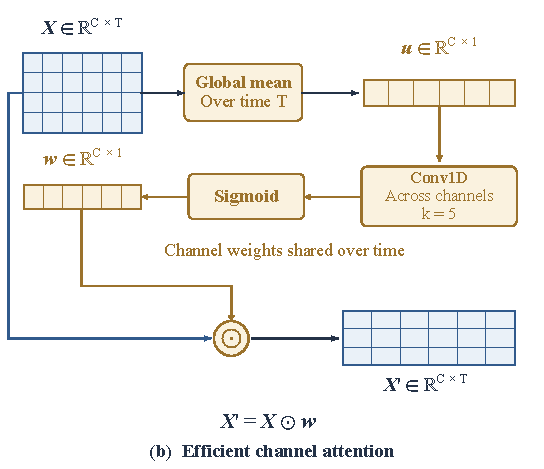
\includegraphics[width=\linewidth]{fig3b_eca_attention_module_revised.pdf}
\end{minipage}

\vspace{0.7em}

\begin{minipage}[t]{0.49\textwidth}
  \centering
  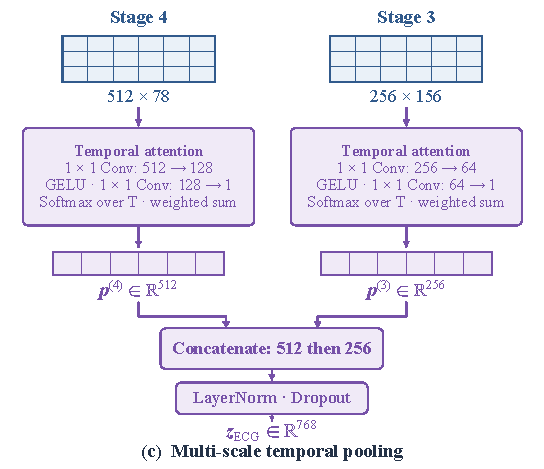
\includegraphics[width=\linewidth]{fig3c_multiscale_temporal_attention_revised.pdf}
\end{minipage}\hfill
\begin{minipage}[t]{0.49\textwidth}
  \centering
  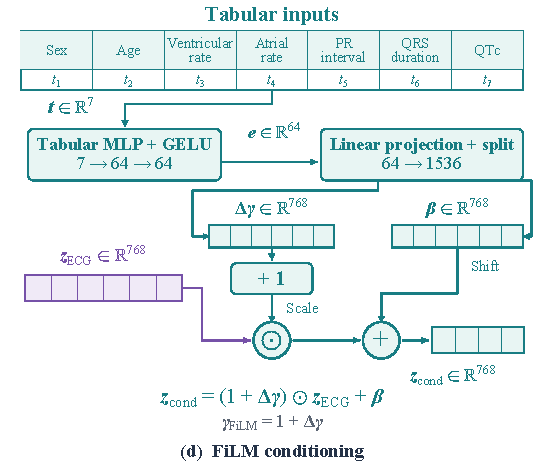
\includegraphics[width=\linewidth]{fig3d_film_conditioning_revised.pdf}
\end{minipage}
\caption{Key downstream modules. (a)--(d), from upper left to lower right: the one-dimensional ECA--ConvNeXt block with GRN, ECA, and DropPath; ECA channel attention with kernel size $k=5$; multiscale temporal attention pooling applied only to Stages 3 and 4; and FiLM conditioning driven by seven tabular variables. }
\label{fig:module_details}
\end{bspcwidefigure}

\subsection{Multiscale temporal representation}
\label{sec:multiscale}

Attention pooling was applied separately to the outputs of Stages 3 and 4. For feature sequence $\mathbf{H}^{(s)}=[\mathbf{h}^{(s)}_1,\ldots,\mathbf{h}^{(s)}_{T_s}]$, the temporal weights and pooled representation are
\begin{align}
a^{(s)}_t &=
\frac{\exp\{g_s(\mathbf{h}^{(s)}_t)\}}
{\sum_{u=1}^{T_s}\exp\{g_s(\mathbf{h}^{(s)}_u)\}},\\
\mathbf{p}^{(s)} &= \sum_{t=1}^{T_s}a^{(s)}_t\mathbf{h}^{(s)}_t,
\label{eq:attention_pool}
\end{align}
where $g_s(\cdot)$ comprises two $1\times1$ convolutions with an intermediate dimension equal to one quarter of the corresponding stage width. Stages 3 and 4 yield 256- and 512-dimensional vectors. The concatenation $[\mathbf{p}^{(4)};\mathbf{p}^{(3)}]$ follows the Stage-4 then Stage-3 order. Layer normalization and dropout with probability 0.2 produce the 768-dimensional ECG representation.

\subsection{Conditioning on tabular inputs}
\label{sec:film}

For each ECG record, the tabular input is $\mathbf{t}\in\mathbb{R}^{7}$. A two-layer multilayer perceptron with GELU activations produces $\mathbf{e}=\mathrm{MLP}(\mathbf{t})\in\mathbb{R}^{64}$. An affine generator produces two 768-dimensional vectors:
\begin{equation}
\begin{bmatrix}\Delta\boldsymbol{\gamma}\\\boldsymbol{\beta}\end{bmatrix}
=\mathbf{W}_{\mathrm{F}}\mathbf{e}+\mathbf{b}_{\mathrm{F}},
\label{eq:film_generator}
\end{equation}
where $\mathbf{W}_{\mathrm{F}}\in\mathbb{R}^{1536\times64}$ and $\mathbf{b}_{\mathrm{F}}\in\mathbb{R}^{1536}$ are learned parameters. The resulting scale offset $\Delta\boldsymbol{\gamma}$ and shift $\boldsymbol{\beta}$ vary with the input. FiLM conditions the ECG representation as
\begin{equation}
\mathbf{z}_{\mathrm{cond}}=
(\mathbf{1}+\Delta\boldsymbol{\gamma})\odot\mathbf{z}_{\mathrm{ECG}}+\boldsymbol{\beta}.
\label{eq:film}
\end{equation}
The original FiLM formulation uses input-conditioned scale and shift functions\cite{perez2018film}; here its effective scale is $\boldsymbol{\gamma}_{\mathrm{FiLM}}=\mathbf{1}+\Delta\boldsymbol{\gamma}$. Both $\mathbf{z}_{\mathrm{ECG}}$ and $\mathbf{z}_{\mathrm{cond}}$ are 768-dimensional vectors, and $\odot$ denotes element-wise multiplication. A linear classifier maps $\mathbf{z}_{\mathrm{cond}}$ to 12 logits.

For a common index, let $y_{12}\equiv y_{\mathrm{SHD}}$ and $\ell_{12}\equiv \ell_{\mathrm{SHD}}$. Training used binary cross-entropy averaged over the 12 binary prediction targets:
\begin{equation}
\mathcal{L}_{\mathrm{BCE}}=-\frac{1}{12}
\sum_{k=1}^{12}
\left[y_k\log\sigma(\ell_k)+(1-y_k)\log(1-\sigma(\ell_k))\right],
\label{eq:bce}
\end{equation}
where $\ell_k$ is the logit for the $k$th prediction target, $\sigma(\cdot)$ is the sigmoid function, and $p_k=\sigma(\ell_k)$ is the corresponding predicted probability. The complete model contains $12{,}149{,}928$ trainable parameters.

\BSPCseparatearchitecturefigures

\subsection{Training and model selection}
\label{sec:training}

Downstream models were trained for up to 100 epochs with a batch size of 64. AdamW used $\beta^{\mathrm{Adam}}_1=0.9$, $\beta^{\mathrm{Adam}}_2=0.999$, an initial learning rate of $10^{-3}$, and weight decay of 0.05. The encoder used a layer-wise learning-rate decay factor of 0.75. The learning rate increased linearly during the first two epochs and followed a cosine schedule thereafter. Gradient norm was clipped at 1.0, and exponential moving-average weights used a decay factor of 0.999.

Training augmentation comprised pointwise Gaussian noise with standard deviation 0.05 and random masking of 10\% of discrete temporal indices, shared across all samples and leads in a batch. Validation and test data were not augmented. Models were selected by validation Overall SHD AUROC, with early stopping after 10 epochs without improvement, and the corresponding exponential moving-average weights were saved. Downstream experiments used random seeds 42, 2026, and 3407 with deterministic training settings. The test set was evaluated only after model selection.

\subsection{Experimental comparisons}
\label{sec:comparisons}

The primary comparison paired the masked-pretrained ECG-FCMAE model (Full) with an identically structured randomly initialized control (Strict). Both used the same seven tabular variables, data splits, loss, optimization, augmentation, training budget, and model-selection rule. Encoder initialization was the experimental factor. Label-efficiency experiments used 1\%, 5\%, 10\%, 30\%, and 100\% of labeled training ECG records. The 1\%--30\% subsets were nested prefixes of one fixed record permutation, and validation and test sets remained fixed.

The input and fusion ablations comprised Full, ECG-only, Concat, and Tabular-only. ECG-only removed the tabular branch and FiLM; Concat retained both input branches but replaced FiLM with simple concatenation; and Tabular-only removed the ECG branch. Strictly matched architecture ablations removed ECA (No ECA), replaced temporal-attention pooling with global average pooling (GAP), or retained only the Stage-4 representation (Stage-4 only), while keeping the 12-lead input, augmentation, data splits, and three downstream seeds fixed. A progressive A--G chain additionally summarized cumulative changes in initialization, ECA, pooling scale, and tabular fusion; its E, F, and G rows reused the ECG-only, Concat, and Full results. Evaluation across prediction targets covered the 11 specific echocardiographic abnormalities and Overall SHD. Reduced-lead analyses used actual channel slicing and selection of the corresponding pretrained stem weights. The configurations were six limb leads, six precordial leads, four anatomical leads (I, II, V1, and V5), Lead I, and Lead II. Each reduced-lead configuration was retrained downstream without dedicated reduced-lead pretraining. Age, sex, race/ethnicity, and clinical-context subgroups were examined descriptively.

\subsection{Statistical analysis}
\label{sec:statistics}

The primary performance metric was AUROC for Overall SHD in the test set. AUPRC was reported as a complementary performance metric sensitive to test-set label prevalence, and performance metrics for each prediction target were reported separately. Macro-11 AUROC was the arithmetic mean over the 11 specific echocardiographic abnormalities, excluding Overall SHD:
\begin{equation}
\mathrm{Macro\mbox{-}11\ AUROC}=\frac{1}{11}
\sum_{k=1}^{11}\mathrm{AUROC}_k.
\label{eq:macro11}
\end{equation}
Macro-11 and Macro-12, which additionally includes Overall SHD, were reported separately.

Means and sample standard deviations across the three downstream training seeds describe training variability. A three-seed probability ensemble was defined as the arithmetic mean of the three predicted probabilities for each patient and prediction target. Confidence intervals for fixed predictions were estimated by 2,000 patient-level percentile-bootstrap replicates. Model differences were paired by applying the same resampled patient indices to both models. Differences were defined as candidate minus reference. Ensemble differences were computed from the observed predictions. Patient-level bootstrap intervals characterize uncertainty from sampling test patients, whereas the three-seed sample standard deviation characterizes variability across training runs. Subgroup analyses were descriptive.

\ifBSPCtwocolumn\else\FloatBarrier\fi
\section{Results}
\label{sec:results}

\subsection{Test cohort and label distribution}
\label{sec:results_cohort}

The test set contained $5{,}442$ patients, of whom $2{,}318$ had a positive ground-truth Overall SHD label, corresponding to a test-set label prevalence of $42.5946\%$. Label prevalence varied across the 11 specific echocardiographic abnormalities. Performance was therefore evaluated separately for Overall SHD and each prediction target, with AUROC, AUPRC, positive ground-truth label counts, and interval width considered jointly for targets with low label prevalence.

\subsection{Pretraining-initialization ablation}
\label{sec:results_primary}

Across three downstream training seeds, Full achieved an Overall SHD AUROC of $0.8521\pm0.0008$, compared with $0.8448\pm0.0001$ for Strict. Corresponding AUPRC values were $0.8249\pm0.0009$ and $0.8149\pm0.0002$, and Macro-11 AUROC was $0.8374\pm0.0020$ and $0.8258\pm0.0032$, respectively (Table~\ref{tab:primary}).

For the three-seed probability ensembles, Overall SHD AUROC was 0.8529 for Full and 0.8468 for Strict. The observed difference was $+0.0061$, with a patient-level paired 95\% CI of $[0.0034,\,0.0088]$. The difference in Overall SHD AUPRC was $+0.0082$ (95\% CI, $[0.0042,\,0.0122]$), and the difference in Macro-11 AUROC was $+0.0099$ (95\% CI, $[0.0049,\,0.0153]$). All three intervals excluded zero, supporting a more useful initialization from masked pretraining under the matched protocol.

\begin{table}[!htbp]
\centering
\BSPCtableformat

\caption{Three-seed results for Full and the identically structured randomly initialized control (Strict). Values are mean$\pm$sample SD across the three downstream training seeds.}
\label{tab:primary}
\begin{tabularx}{\linewidth}{@{}Ycc@{}}
\toprule
Metric & Full & Strict \\
\midrule
SHD AUROC & 0.8521$\pm$0.0008 & 0.8448$\pm$0.0001 \\
SHD AUPRC & 0.8249$\pm$0.0009 & 0.8149$\pm$0.0002 \\
Macro-11 AUROC & 0.8374$\pm$0.0020 & 0.8258$\pm$0.0032 \\
\bottomrule
\end{tabularx}

\end{table}

\BSPCseparateresultfloatgroups

\subsection{Label efficiency}
\label{sec:results_label_efficiency}

Pretraining improved performance at all five labeled-record fractions (Table~\ref{tab:label_efficiency}; Figure~\ref{fig:label_efficiency}). At 1\%, three-seed AUROC was $0.8003\pm0.0035$ for the pretrained model (SSL) and $0.7641\pm0.0130$ for random initialization (Scratch). At 100\%, the corresponding values were $0.8521\pm0.0008$ and $0.8448\pm0.0001$. Scratch showed its largest between-seed dispersion at 1\%.

The SSL$-$Scratch AUROC differences between the three-seed probability ensembles were $+0.0323$, $+0.0196$, $+0.0127$, $+0.0055$, and $+0.0061$ at 1\%, 5\%, 10\%, 30\%, and 100\%, respectively. Every paired 95\% CI excluded zero (Table~\ref{tab:label_paired}). The corresponding AUPRC differences were $+0.0579$, $+0.0339$, $+0.0204$, $+0.0112$, and $+0.0082$, and their intervals also excluded zero. The AUROC gain was largest at 1\% and decreased overall as label availability increased, with a small increase from 30\% to 100\%; the AUPRC gain decreased across all five fractions.

\begin{table}[!htbp]
\centering
\BSPCtableformat

\caption{Results at different fractions of labeled training ECG records. Values are mean$\pm$sample SD across the three downstream training seeds. The 100\% condition reuses Full and Strict.}
\label{tab:label_efficiency}
\begin{tabularx}{\linewidth}{@{}Ycc@{}}
\toprule
\multicolumn{3}{l}{\textit{(a) Overall SHD AUROC}} \\
Fraction & SSL & Scratch \\
\midrule
1\% & 0.8003$\pm$0.0035 & 0.7641$\pm$0.0130 \\
5\% & 0.8250$\pm$0.0008 & 0.8001$\pm$0.0023 \\
10\% & 0.8350$\pm$0.0013 & 0.8181$\pm$0.0028 \\
30\% & 0.8447$\pm$0.0005 & 0.8365$\pm$0.0027 \\
100\% & 0.8521$\pm$0.0008 & 0.8448$\pm$0.0001 \\
\midrule
\multicolumn{3}{l}{\textit{(b) Overall SHD AUPRC}} \\
Fraction & SSL & Scratch \\
\midrule
1\% & 0.7609$\pm$0.0054 & 0.6978$\pm$0.0215 \\
5\% & 0.7983$\pm$0.0012 & 0.7554$\pm$0.0054 \\
10\% & 0.8084$\pm$0.0013 & 0.7818$\pm$0.0037 \\
30\% & 0.8185$\pm$0.0006 & 0.8037$\pm$0.0029 \\
100\% & 0.8249$\pm$0.0009 & 0.8149$\pm$0.0002 \\
\bottomrule
\end{tabularx}

\end{table}

\begin{table}[!htbp]
\centering
\BSPCtableformat

\caption{Label-efficiency differences between three-seed probability ensembles. Values are observed SSL$-$Scratch differences with patient-level paired 95\% CIs from 2,000 bootstrap replicates. The 100\% row uses the label-efficiency bootstrap analysis.}
\label{tab:label_paired}
\begin{tabularx}{\linewidth}{@{}lZZ@{}}
\toprule
Fraction & $\Delta$ SHD AUROC & $\Delta$ SHD AUPRC \\
\midrule
1\% & \shortstack{$0.0323$\\$[0.0239,\,0.0408]$} & \shortstack{$0.0579$\\$[0.0453,\,0.0707]$} \\
5\% & \shortstack{$0.0196$\\$[0.0134,\,0.0258]$} & \shortstack{$0.0339$\\$[0.0251,\,0.0425]$} \\
10\% & \shortstack{$0.0127$\\$[0.0077,\,0.0176]$} & \shortstack{$0.0204$\\$[0.0128,\,0.0282]$} \\
30\% & \shortstack{$0.0055$\\$[0.0017,\,0.0093]$} & \shortstack{$0.0112$\\$[0.0057,\,0.0167]$} \\
100\% & \shortstack{$0.0061$\\$[0.0034,\,0.0088]$} & \shortstack{$0.0082$\\$[0.0044,\,0.0122]$} \\
\bottomrule
\end{tabularx}

\end{table}
\begin{bspclabelefficiencyfigure}
\centering
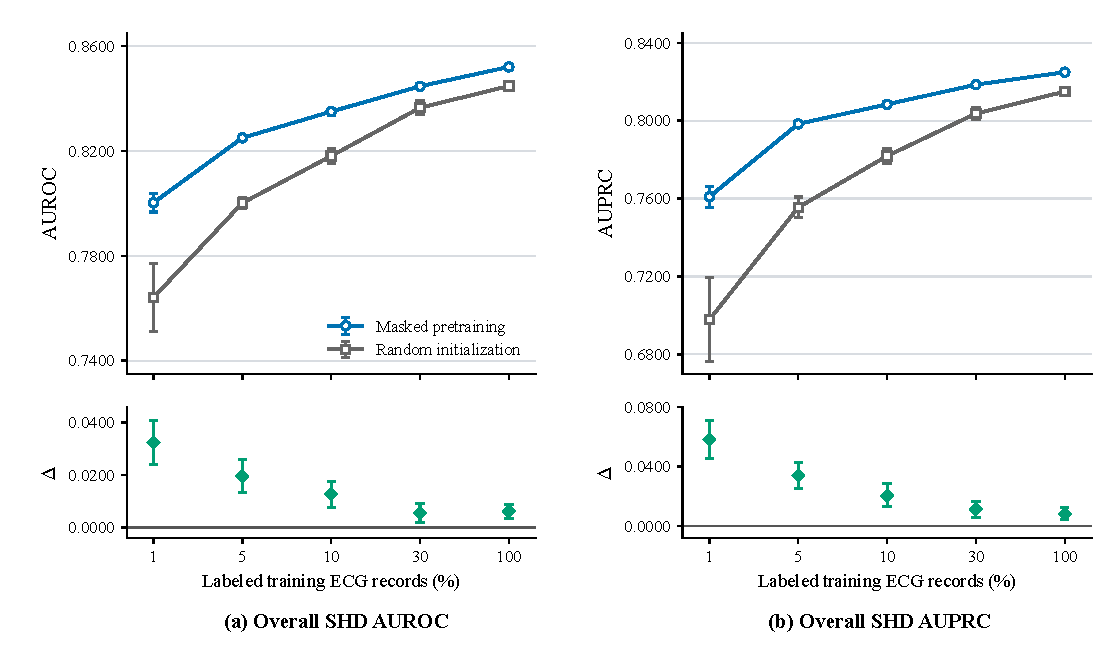
\includegraphics[width=0.8800\textwidth]{fig4_label_efficiency_revised.pdf}
\caption{Overall SHD performance across fractions of labeled training ECG records. (a) AUROC and (b) AUPRC at 1\%, 5\%, 10\%, 30\%, and 100\% of labeled training records. Upper panels show the mean across three downstream training seeds; vertical bars denote sample standard deviation across seeds. Lower strips show the observed masked-pretraining minus random-initialization difference between three-seed probability ensembles; vertical bars denote patient-level paired 95\% confidence intervals from 2,000 percentile-bootstrap replicates. Fractions were defined over training ECG records. The 100\% condition reused Full and Strict, and the displayed 100\% intervals are from the label-efficiency bootstrap analysis.}
\label{fig:label_efficiency}
\end{bspclabelefficiencyfigure}

\BSPCseparateresultfloatgroups

\subsection{Input and fusion ablations}
\label{sec:results_structured}

The input and fusion ablations showed that ECG waveforms provided the principal discriminative information, while the seven tabular variables added complementary information in Full (Table~\ref{tab:modalities}). Three-seed Overall SHD AUROC was $0.8521\pm0.0008$ for Full, $0.8466\pm0.0006$ for ECG-only, and $0.7587\pm0.0006$ for Tabular-only.

Concat achieved a three-seed AUROC of $0.8505\pm0.0008$, close to Full.

\begin{table}[!htbp]
\centering
\BSPCtableformat

\caption{Three-seed test results for the input and fusion ablations. Full uses ECGs, seven tabular variables, and FiLM; ECG-only removes the tabular branch and FiLM; Concat replaces FiLM with simple concatenation; and Tabular-only removes the ECG branch.}
\label{tab:modalities}
\begin{tabularx}{\linewidth}{@{}Yccc@{}}
\toprule
Model & SHD AUROC & SHD AUPRC & \shortstack{Macro-11\\AUROC} \\
\midrule
Full & 0.8521$\pm$0.0008 & 0.8249$\pm$0.0009 & 0.8374$\pm$0.0020 \\
ECG-only & 0.8466$\pm$0.0006 & 0.8214$\pm$0.0006 & 0.8297$\pm$0.0025 \\
Concat & 0.8505$\pm$0.0008 & 0.8224$\pm$0.0009 & 0.8348$\pm$0.0002 \\
Tabular-only & 0.7587$\pm$0.0006 & 0.7002$\pm$0.0018 & 0.7281$\pm$0.0018 \\
\bottomrule
\end{tabularx}

\end{table}

\subsection{Architecture-component ablations}
\label{sec:results_architecture_ablation}

The component ablations produced point estimates close to Full (Table~\ref{tab:architecture_ablation}). Overall SHD AUROC was $0.8519\pm0.0003$ without ECA, $0.8517\pm0.0004$ with GAP, and $0.8517\pm0.0005$ with Stage 4 alone, compared with $0.8521\pm0.0008$ for Full.

The cumulative A--G chain ranged from $0.8390\pm0.0021$ AUROC for A (random initialization, no ECA, Stage-4 GAP, and no tabular fusion) to $0.8521\pm0.0008$ for G (Full). Table~\ref{tab:component_chain} summarizes the cumulative configurations and their mean performance.

\begin{table}[!htbp]
\centering
\BSPCtableformat

\caption{Strictly matched architecture-component ablations. Values are three-seed mean$\pm$sample SD. Strict changes only the pretrained initialization; No ECA removes ECA; GAP replaces temporal-attention pooling with global average pooling; and Stage-4 only removes the Stage-3 aggregation path.}
\label{tab:architecture_ablation}
\begin{tabularx}{\linewidth}{@{}Yccc@{}}
\toprule
Configuration & SHD AUROC & SHD AUPRC & \shortstack{Macro-11\\AUROC} \\
\midrule
Full & 0.8521$\pm$0.0008 & 0.8249$\pm$0.0009 & 0.8374$\pm$0.0020 \\
\BSPCstrictnopretraining & 0.8448$\pm$0.0001 & 0.8149$\pm$0.0002 & 0.8258$\pm$0.0032 \\
No ECA & 0.8519$\pm$0.0003 & 0.8262$\pm$0.0014 & 0.8366$\pm$0.0003 \\
GAP & 0.8517$\pm$0.0004 & 0.8240$\pm$0.0012 & 0.8366$\pm$0.0019 \\
Stage-4 only & 0.8517$\pm$0.0005 & 0.8253$\pm$0.0017 & 0.8379$\pm$0.0007 \\
\bottomrule
\end{tabularx}

\end{table}

\begin{bspcwidetable}[!htbp]
\centering
\BSPCtableformat

\caption{Progressive A--G component chain. Each row gives a cumulative configuration and its three-seed mean$\pm$sample SD. E, F, and G reuse ECG-only, Concat, and Full, respectively.}
\label{tab:component_chain}
% Usable column widths: 6%, 16%, 5%, 17%, 8%, 16%, 16%, 16%.
% The eight X-column weights sum to 8, preserving the full table width.
\begin{tabularx}{\textwidth}{@{}
  >{\hsize=0.48\hsize\linewidth=\hsize\centering\arraybackslash}X
  >{\hsize=1.28\hsize\linewidth=\hsize\raggedright\arraybackslash}X
  >{\hsize=0.40\hsize\linewidth=\hsize\centering\arraybackslash}X
  >{\hsize=1.36\hsize\linewidth=\hsize\raggedright\arraybackslash}X
  >{\hsize=0.64\hsize\linewidth=\hsize\centering\arraybackslash}X
  *{3}{>{\hsize=1.28\hsize\linewidth=\hsize\centering\arraybackslash}X}
@{}}
\toprule
Group & Initialization & ECA & Pooling / scale & \shortstack{Tabular\\fusion} & \shortstack{SHD\\AUROC} & \shortstack{SHD\\AUPRC} & \shortstack{Macro-11\\AUROC} \\
\midrule
A & Scratch & Off & Stage-4 GAP & None & 0.8390$\pm$0.0021 & 0.8106$\pm$0.0029 & 0.8236$\pm$0.0032 \\
B & FCMAE no-ECA & Off & Stage-4 GAP & None & 0.8459$\pm$0.0008 & 0.8221$\pm$0.0006 & 0.8290$\pm$0.0011 \\
C & FCMAE\allowbreak(ECA) & On & Stage-4 GAP & None & 0.8466$\pm$0.0003 & 0.8211$\pm$0.0011 & 0.8299$\pm$0.0006 \\
D & FCMAE\allowbreak(ECA) & On & Stage-4 attention & None & 0.8470$\pm$0.0006 & 0.8218$\pm$0.0009 & 0.8307$\pm$0.0005 \\
E & FCMAE\allowbreak(ECA) & On & Stage-3/4 attention & None & 0.8466$\pm$0.0006 & 0.8214$\pm$0.0006 & 0.8297$\pm$0.0025 \\
F & FCMAE\allowbreak(ECA) & On & Stage-3/4 attention & Concat & 0.8505$\pm$0.0008 & 0.8224$\pm$0.0009 & 0.8348$\pm$0.0002 \\
G & FCMAE\allowbreak(ECA) & On & Stage-3/4 attention & FiLM & 0.8521$\pm$0.0008 & 0.8249$\pm$0.0009 & 0.8374$\pm$0.0020 \\
\bottomrule
\end{tabularx}

\end{bspcwidetable}

\BSPCseparateresultfloatgroups

\subsection{Comparison with reported EchoNext models}
\label{sec:results_published_comparison}

Prior EchoNext studies report both the Overall SHD prediction target and Macro-11 AUROC across the 11 specific abnormalities. EchoNext-Mini uses the 12-lead ECG and seven tabular variables, whereas the interpretable generalized additive model uses 71 ECG foundation-model predictors with the same seven tabular variables; their reported Overall SHD AUROCs were 0.8200 and 0.8280, respectively\cite{hughes2026echonextmini,zhou2026gamshd}. The unified EchoNext benchmark evaluated fine-tuned foundation models and supervised models under the same label system, with ECG-only Macro-11 AUROC ranging from 0.7720 to 0.8310\cite{almasud2026benchmark}. Table~\ref{tab:published_comparison} places these reported values alongside the three-seed results for ECG-FCMAE.

\begin{table}[!htbp]
\centering
\BSPCtableformat

\caption{Reported EchoNext results and ECG-FCMAE. Literature values follow their original study protocols; our results are mean$\pm$sample SD across three seeds. T denotes seven tabular variables; P denotes 71 ECG foundation-model predictors.}
\label{tab:published_comparison}
\begin{tabularx}{\linewidth}{@{}Yp{0.1900\linewidth}r@{}}
\toprule
Method & Input & AUROC \\
\midrule
\multicolumn{3}{@{}l}{\textit{(a) Overall SHD AUROC}} \\
EchoNext-Mini\cite{hughes2026echonextmini} & ECG + T & 0.8200 \\
Interpretable GAM\cite{zhou2026gamshd} & P + T & 0.8280 \\
\midrule
\textbf{ECG-FCMAE (Ours)} & ECG + T & 0.8521$\pm$0.0008 \\
\midrule
\multicolumn{3}{@{}l}{\textit{(b) Macro-11 AUROC}} \\
\multicolumn{3}{@{}l}{Fine-tuned foundation models\cite{almasud2026benchmark}} \\
ECGFounder & ECG & 0.8170 \\
ECG-JEPA & ECG & 0.8170 \\
ST-MEM & ECG & 0.8160 \\
MERL & ECG & 0.8220 \\
ECGFM-KED & ECG & 0.8060 \\
HuBERT-ECG & ECG & 0.7920 \\
ECG-FM & ECG & 0.7720 \\
ECG-CPC & ECG & 0.8310 \\
\addlinespace
\multicolumn{3}{@{}l}{Supervised models\cite{almasud2026benchmark}} \\
S4 & ECG & 0.8190 \\
Net1D & ECG & 0.8030 \\
\midrule
\textbf{ECG-FCMAE, ECG-only (Ours)} & ECG & 0.8297$\pm$0.0025 \\
\textbf{ECG-FCMAE (Ours)} & ECG + T & 0.8374$\pm$0.0020 \\
\bottomrule
\end{tabularx}

\end{table}

ECG-FCMAE achieved a three-seed mean Overall SHD AUROC of $0.8521\pm0.0008$. Its ECG-only variant achieved Macro-11 AUROC of $0.8297\pm0.0025$, close to the 0.8310 reported for ECG-CPC in the unified benchmark. Adding seven tabular variables yielded $0.8374\pm0.0020$ for the complete model.

\BSPCseparateresultfloatgroups

\subsection{Performance across prediction targets}
\label{sec:results_endpoints}

The Full three-seed probability ensemble showed marked performance heterogeneity across prediction targets (Table~\ref{tab:endpoints}; Figure~\ref{fig:endpoints}). Across the 11 specific echocardiographic abnormalities, AUROC ranged from 0.7717 for moderate-or-greater aortic regurgitation to 0.9081 for LVEF $\leq45\%$, whereas AUPRC ranged from 0.0514 to 0.7470 for the same prediction targets. AUROC was 0.8995 for moderate-or-greater right ventricular systolic dysfunction and 0.8895 for moderate-or-greater aortic stenosis. Moderate-or-greater pulmonary regurgitation, moderate-or-greater aortic regurgitation, and moderate or large pericardial effusion had low AUPRC values and wide intervals, indicating substantial uncertainty for these prediction targets with low label prevalence.

\begin{bspcwidefigure}[t]
\centering
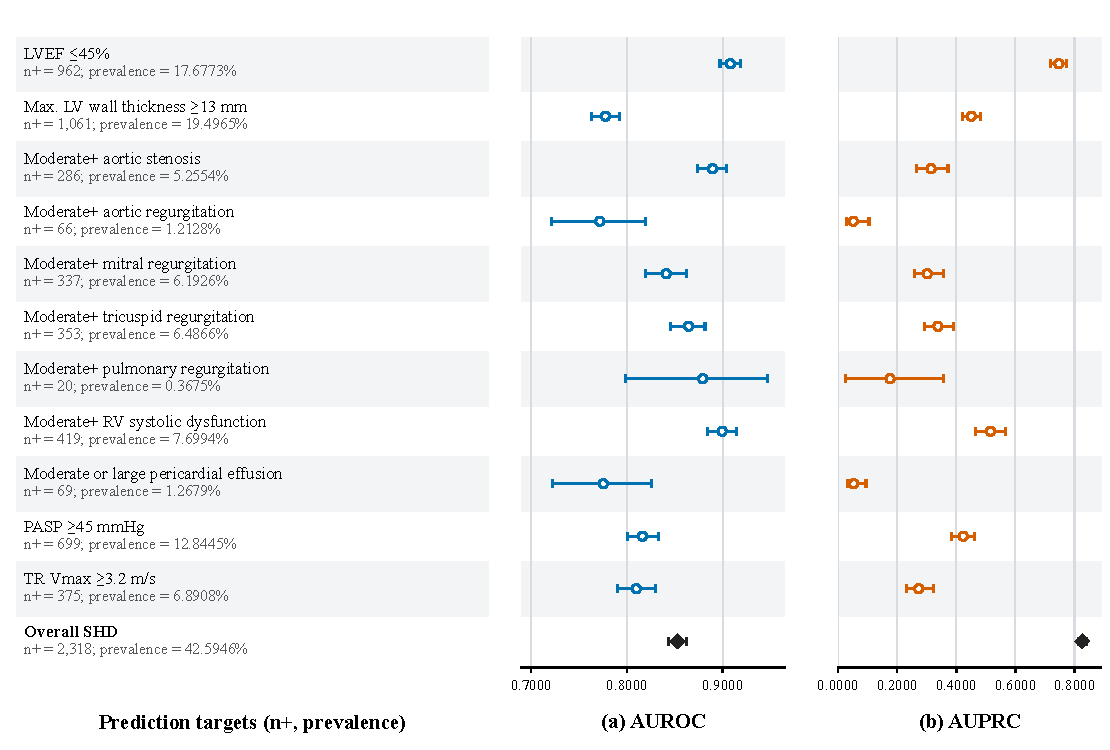
\includegraphics[width=0.9600\textwidth]{fig5_endpoint_performance_revised.pdf}
\caption{Performance across prediction targets for the Full three-seed probability ensemble. (a) AUROC and (b) AUPRC for 11 specific echocardiographic abnormalities and Overall SHD. Points are observed ensemble estimates and horizontal bars are patient-level 95\% confidence intervals from 2,000 bootstrap replicates. Left labels report the positive ground-truth label count and test-set label prevalence in the fixed 5,442-patient test set; the Overall SHD row is shown with a diamond. Positive-label counts and prevalence accompany the prevalence-sensitive AUPRC estimates.}
\label{fig:endpoints}
\end{bspcwidefigure}

\begin{bspcwidetable}[!tbp]
\centering
\BSPCtableformat

\caption{Results across prediction targets for the Full three-seed probability ensemble. Confidence intervals are patient-level 95\% intervals from 2,000 bootstrap replicates.}
\label{tab:endpoints}
\begin{tabularx}{\textwidth}{Ycc}
\toprule
Prediction target & AUROC (95\% CI) & AUPRC (95\% CI) \\
\midrule
LVEF $\leq45\%$ & 0.9081 $[0.8973,\,0.9189]$ & 0.7470 $[0.7194,\,0.7728]$ \\
Maximum diastolic thickness of the interventricular septum or left ventricular posterior wall $\geq13$~mm & 0.7775 $[0.7628,\,0.7921]$ & 0.4508 $[0.4207,\,0.4821]$ \\
Moderate-or-greater aortic stenosis & 0.8895 $[0.8734,\,0.9044]$ & 0.3146 $[0.2665,\,0.3719]$ \\
Moderate-or-greater aortic regurgitation & 0.7717 $[0.7208,\,0.8196]$ & 0.0514 $[0.0301,\,0.1047]$ \\
Moderate-or-greater mitral regurgitation & 0.8410 $[0.8190,\,0.8621]$ & 0.3015 $[0.2580,\,0.3554]$ \\
Moderate-or-greater tricuspid regurgitation & 0.8645 $[0.8458,\,0.8816]$ & 0.3378 $[0.2930,\,0.3906]$ \\
Moderate-or-greater pulmonary regurgitation & 0.8793 $[0.7988,\,0.9474]$ & 0.1759 $[0.0243,\,0.3579]$ \\
Moderate-or-greater right ventricular systolic dysfunction & 0.8995 $[0.8838,\,0.9145]$ & 0.5157 $[0.4656,\,0.5664]$ \\
Moderate or large pericardial effusion & 0.7752 $[0.7221,\,0.8258]$ & 0.0530 $[0.0337,\,0.0945]$ \\
PASP $\geq45$ mmHg & 0.8162 $[0.8004,\,0.8326]$ & 0.4233 $[0.3839,\,0.4608]$ \\
TR Vmax $\geq3.2$ m/s & 0.8098 $[0.7900,\,0.8298]$ & 0.2728 $[0.2311,\,0.3216]$ \\
Overall SHD & 0.8529 $[0.8431,\,0.8627]$ & 0.8263 $[0.8120,\,0.8403]$ \\
\bottomrule
\end{tabularx}

\end{bspcwidetable}

\BSPCkeependpointorder

\subsection{Reduced-lead analysis}
\label{sec:results_reduced_leads}

All reduced-lead models were retrained downstream after actual channel slicing. Three-seed Overall SHD AUROC was $0.8463\pm0.0003$ for the six precordial leads (Precordial-6) and $0.8465\pm0.0006$ for the I/II/V1/V5 configuration (Anatomical-4), making these the closest of the five configurations to 12-lead Full. AUROC was $0.8322\pm0.0016$ for Limb-6, $0.8245\pm0.0005$ for Lead-I, and $0.8196\pm0.0005$ for Lead-II.

Table~\ref{tab:reduced_summary} summarizes performance across the five reduced-lead configurations. The lower mean AUROC values quantify the decrease associated with fewer input channels.

\begin{table}[!htbp]
\centering
\BSPCtableformat

\caption{Reduced-lead test performance, reported as three-seed mean$\pm$sample SD. Limb-6 uses I, II, III, aVR, aVL, and aVF; Precordial-6 uses V1--V6; Anatomical-4 uses I, II, V1, and V5.}
\label{tab:reduced_summary}
\begin{tabularx}{\linewidth}{@{}Yccc@{}}
\toprule
Configuration & SHD AUROC & SHD AUPRC & \shortstack{Macro-11\\AUROC} \\
\midrule
Limb-6 & 0.8322$\pm$0.0016 & 0.8007$\pm$0.0024 & 0.8087$\pm$0.0043 \\
Precordial-6 & 0.8463$\pm$0.0003 & 0.8192$\pm$0.0005 & 0.8306$\pm$0.0011 \\
Anatomical-4 & 0.8465$\pm$0.0006 & 0.8208$\pm$0.0013 & 0.8314$\pm$0.0012 \\
Lead-I & 0.8245$\pm$0.0005 & 0.7962$\pm$0.0002 & 0.7942$\pm$0.0052 \\
Lead-II & 0.8196$\pm$0.0005 & 0.7783$\pm$0.0005 & 0.7857$\pm$0.0024 \\
\bottomrule
\end{tabularx}

\end{table}

\subsection{Prespecified subgroup analysis}
\label{sec:results_subgroups}

Full exceeded Strict in AUROC point estimates in 15 of 16 prespecified subgroups, and nine patient-level paired 95\% CIs excluded zero (Table~\ref{tab:subgroups}). The largest difference was in patients aged 70--79 years, $+0.0134$ (95\% CI, $[0.0066,\,0.0204]$), while the Asian subgroup had a difference of $-0.0022$ (95\% CI, $[-0.0210,\,0.0152]$). Smaller subgroups, including Asian and Procedural, had wider intervals. Subgroup AUPRC is presented with the corresponding SHD prevalence.

\begin{bspcwidetable}[!htbp]
\centering
\BSPCtableformat

\caption{Three-seed probability-ensemble performance in prespecified subgroups. Cells report estimates with patient-level 95\% CIs from 2,000 bootstrap replicates; $\Delta$ AUROC is Full$-$Strict. Counts are patients / SHD-positive patients, and prevalence is their ratio. AUPRC is reported alongside subgroup prevalence.}
\label{tab:subgroups}
% Usable column widths: 18%, 10%, 10%, 15%, 15%, 15%, 17%.
% The seven X-column weights sum to 7; the difference column allows for minus signs.
\begin{tabularx}{\textwidth}{@{}
  >{\hsize=1.26\hsize\linewidth=\hsize\raggedright\arraybackslash}X
  *{2}{>{\hsize=0.70\hsize\linewidth=\hsize\centering\arraybackslash}X}
  *{3}{>{\hsize=1.05\hsize\linewidth=\hsize\centering\arraybackslash}X}
  >{\hsize=1.19\hsize\linewidth=\hsize\centering\arraybackslash}X
@{}}
\toprule
Subgroup & $n/n_+$ & Prevalence & \shortstack{Strict\\AUROC} & \shortstack{Full\\AUROC} & \shortstack{Full\\AUPRC} & $\Delta$ AUROC \\
\midrule
\multicolumn{7}{@{}l}{\textit{Age}} \\
18--59 & 2124/671 & 0.3159 & \shortstack{$0.8560$\\$[0.8390,\,0.8730]$} & \shortstack{$0.8610$\\$[0.8440,\,0.8780]$} & \shortstack{$0.7780$\\$[0.7460,\,0.8060]$} & \shortstack{$0.0048$\\$[-0.0003,\,0.0096]$} \\
60--69 & 1318/524 & 0.3976 & \shortstack{$0.8390$\\$[0.8170,\,0.8600]$} & \shortstack{$0.8480$\\$[0.8260,\,0.8680]$} & \shortstack{$0.8080$\\$[0.7760,\,0.8380]$} & \shortstack{$0.0086$\\$[0.0025,\,0.0145]$} \\
70--79 & 1154/578 & 0.5009 & \shortstack{$0.8010$\\$[0.7760,\,0.8250]$} & \shortstack{$0.8150$\\$[0.7890,\,0.8380]$} & \shortstack{$0.8380$\\$[0.8100,\,0.8630]$} & \shortstack{$0.0134$\\$[0.0066,\,0.0204]$} \\
80+ & 846/545 & 0.6442 & \shortstack{$0.7860$\\$[0.7540,\,0.8160]$} & \shortstack{$0.7890$\\$[0.7570,\,0.8180]$} & \shortstack{$0.8780$\\$[0.8530,\,0.9010]$} & \shortstack{$0.0029$\\$[-0.0064,\,0.0125]$} \\
\midrule
\multicolumn{7}{@{}l}{\textit{Sex}} \\
Female & 2731/1001 & 0.3665 & \shortstack{$0.8470$\\$[0.8320,\,0.8620]$} & \shortstack{$0.8520$\\$[0.8370,\,0.8660]$} & \shortstack{$0.7890$\\$[0.7640,\,0.8120]$} & \shortstack{$0.0049$\\$[0.0007,\,0.0090]$} \\
Male & 2711/1317 & 0.4858 & \shortstack{$0.8410$\\$[0.8260,\,0.8550]$} & \shortstack{$0.8480$\\$[0.8340,\,0.8630]$} & \shortstack{$0.8520$\\$[0.8330,\,0.8690]$} & \shortstack{$0.0077$\\$[0.0038,\,0.0116]$} \\
\midrule
\multicolumn{7}{@{}l}{\textit{Race/Ethnicity}} \\
Hispanic & 1649/620 & 0.3760 & \shortstack{$0.8470$\\$[0.8280,\,0.8660]$} & \shortstack{$0.8540$\\$[0.8350,\,0.8710]$} & \shortstack{$0.8050$\\$[0.7770,\,0.8320]$} & \shortstack{$0.0064$\\$[0.0015,\,0.0117]$} \\
White & 1569/656 & 0.4181 & \shortstack{$0.8370$\\$[0.8180,\,0.8580]$} & \shortstack{$0.8430$\\$[0.8240,\,0.8630]$} & \shortstack{$0.8110$\\$[0.7830,\,0.8380]$} & \shortstack{$0.0061$\\$[0.0005,\,0.0115]$} \\
Black & 846/405 & 0.4787 & \shortstack{$0.8470$\\$[0.8200,\,0.8710]$} & \shortstack{$0.8520$\\$[0.8250,\,0.8770]$} & \shortstack{$0.8550$\\$[0.8250,\,0.8840]$} & \shortstack{$0.0055$\\$[-0.0011,\,0.0123]$} \\
Asian & 153/70 & 0.4575 & \shortstack{$0.8480$\\$[0.7840,\,0.9070]$} & \shortstack{$0.8460$\\$[0.7820,\,0.9050]$} & \shortstack{$0.8240$\\$[0.7310,\,0.9010]$} & \shortstack{$-0.0022$\\$[-0.0210,\,0.0152]$} \\
Other & 457/200 & 0.4376 & \shortstack{$0.8480$\\$[0.8130,\,0.8820]$} & \shortstack{$0.8530$\\$[0.8200,\,0.8860]$} & \shortstack{$0.8300$\\$[0.7810,\,0.8780]$} & \shortstack{$0.0055$\\$[-0.0043,\,0.0161]$} \\
Unknown & 768/367 & 0.4779 & \shortstack{$0.8540$\\$[0.8270,\,0.8800]$} & \shortstack{$0.8630$\\$[0.8360,\,0.8870]$} & \shortstack{$0.8530$\\$[0.8160,\,0.8870]$} & \shortstack{$0.0085$\\$[0.0011,\,0.0158]$} \\
\midrule
\multicolumn{7}{@{}l}{\textit{Clinical context}} \\
Emergency & 1971/788 & 0.3998 & \shortstack{$0.8510$\\$[0.8350,\,0.8680]$} & \shortstack{$0.8580$\\$[0.8420,\,0.8740]$} & \shortstack{$0.8120$\\$[0.7850,\,0.8380]$} & \shortstack{$0.0064$\\$[0.0018,\,0.0108]$} \\
Inpatient & 2203/1156 & 0.5247 & \shortstack{$0.8220$\\$[0.8040,\,0.8400]$} & \shortstack{$0.8290$\\$[0.8120,\,0.8450]$} & \shortstack{$0.8560$\\$[0.8370,\,0.8730]$} & \shortstack{$0.0066$\\$[0.0014,\,0.0118]$} \\
Outpatient & 1059/271 & 0.2559 & \shortstack{$0.8300$\\$[0.8000,\,0.8580]$} & \shortstack{$0.8370$\\$[0.8060,\,0.8650]$} & \shortstack{$0.7140$\\$[0.6620,\,0.7640]$} & \shortstack{$0.0068$\\$[-0.0003,\,0.0137]$} \\
Procedural & 209/103 & 0.4928 & \shortstack{$0.8380$\\$[0.7850,\,0.8880]$} & \shortstack{$0.8500$\\$[0.7950,\,0.8970]$} & \shortstack{$0.8370$\\$[0.7640,\,0.9000]$} & \shortstack{$0.0115$\\$[-0.0047,\,0.0284]$} \\
\bottomrule
\end{tabularx}

\end{bspcwidetable}

\section{Discussion}
\label{sec:discussion}

\subsection{Principal findings and ECG representation learning}
\label{sec:discussion_findings}

Masked pretraining improved Overall SHD AUROC, AUPRC, and Macro-11 AUROC relative to random initialization in EchoNext. The Overall SHD AUROC difference between three-seed probability ensembles was $+0.0061$, with a patient-level paired 95\% CI above zero. These results support reconstruction of unlabeled ECGs as an effective initialization for subsequent SHD discrimination.

The architecture ablations yielded small point differences after removing ECA, replacing attention pooling with GAP, or retaining Stage 4 alone. The A--G chain complements these single-factor comparisons by describing cumulative design changes relative to Full.

Shared temporal-patch masking requires the encoder to combine unmasked temporal context with synchronized lead information when reconstructing missing segments. Previous masked ECG models also use temporal or lead-wise context for downstream transfer\cite{zhang2023maefe,na2024stmem,ran_joint_masking_2024,sawano_masked_lvsd_2024}. The matched comparison and label-efficiency results are consistent with reconstruction learning reusable ECG representations before exposure to downstream labels.

\subsection{Label efficiency and relation to previous ECG self-supervised learning}
\label{sec:discussion_label_efficiency}

Pretraining improved label efficiency across the five labeled-record fractions. Paired CIs for both SSL$-$Scratch AUROC and AUPRC excluded zero throughout 1\%--100\%. The AUROC difference was largest at 1\% ($+0.0323$) and decreased overall to $+0.0061$ at 100\%, with a small increase from 30\% to 100\%.

ECG self-supervised studies have learned representations through cross-view contrast, lead relationships, transformation recognition, and masked reconstruction\cite{kiyasseh2021clocs,mehari2022ssl,oh2022leadagnostic,zhang_reverse_2023,zhang2023maefe,na2024stmem}. Masked pretraining has also been evaluated for left ventricular systolic dysfunction under limited labels\cite{sawano_masked_lvsd_2024}. Our evaluation connects these representation-learning objectives to a 12-target SHD task through an architecture-matched initialization comparison and nested fractions of labeled ECG records.

\subsection{Tabular information, performance heterogeneity across prediction targets, and reduced-lead inputs}
\label{sec:discussion_secondary}

The input ablations identify ECG waveforms as the principal source of discriminative information: ECG-only exceeded Tabular-only, and Full exceeded ECG-only. Seven tabular variables therefore added complementary information. Related multimodal ECG studies also link fusion performance to the input representation and prediction target\cite{jiang_multimodal_lqts_2024,narotamo_multimodal_2024}. FiLM and concatenation produced close mean performance estimates.

Performance varied substantially across prediction targets in AUROC, AUPRC, and interval width. LVEF $\leq45\%$ and moderate-or-greater right ventricular systolic dysfunction had high AUROC values, whereas moderate-or-greater aortic regurgitation, moderate-or-greater pulmonary regurgitation, and moderate or large pericardial effusion had low AUPRC values. Target-level estimates, test-set label prevalence, and interval width together characterize this heterogeneity.

Reducing the input channels decreased Overall SHD AUROC. Precordial-6 and Anatomical-4 retained the most performance among the five reduced-lead configurations. These retrained models characterize the sensitivity of SHD discrimination to channel availability and complement previous reduced-lead classification and single-lead SHD studies\cite{le_lightx3ecg_2023,aminorroaya_adapt_shd_2025}.

\subsection{Clinical relevance and limitations}
\label{sec:discussion_clinical_limitations}

ECG-derived SHD probabilities offer a basis for prioritizing echocardiography, the confirmatory examination for structural abnormalities. External calibration, decision analysis, and prospective workflow evaluation can quantify the value of this prioritization in clinical practice.

The evaluation used a single-center retrospective paired cohort. Label-efficiency subsets were sampled by ECG record, with repeated records permitted in training. The three downstream seeds shared one pretrained checkpoint, so their dispersion estimates downstream training variability. Age and sex served as both subgroup definitions and tabular inputs; subgroup estimates describe performance within these observed groups.

The data release provides processed arrays but omits the complete cohort-generation and repeated-echocardiogram selection workflow, raw-waveform-to-array code, filter parameters, preprocessing fitting population and statistics, and tabular scaling and missing-value implementation. These missing upstream details limit reconstruction of the complete data pipeline. Independent pretraining runs and external cohorts would assess pretraining variability and transportability, while prospective evaluation would assess calibration and decision utility.

\FloatBarrier
\section{Conclusion}
\label{sec:conclusion}

ECG-FCMAE improved 12-lead ECG detection of echocardiography-defined SHD in EchoNext. Compared with random initialization, the three-seed probability ensemble gained $0.0061$ Overall SHD AUROC (patient-level paired 95\% CI, $[0.0034,\,0.0088]$). Pretraining improved performance across 1\%--100\% of labeled training records, with the largest gain at 1\%. Input ablations showed that ECG waveforms carried the principal discriminative information and that tabular variables added complementary value. Target-specific and reduced-lead analyses characterized how performance varied with the prediction task and available channels.
